\documentclass{standalone}
\usepackage{tikz}
\usetikzlibrary{arrows}
\tikzset{
  treenode/.style = {align=center, inner sep=0pt, text centered,
    font=\sffamily},
  arn_n/.style = {treenode, circle, white, font=\sffamily\bfseries, draw=black,
    fill=black, text width=1.5em},% arbre rouge noir, noeud noir
  arn_r/.style = {treenode, circle, red, draw=red,
    text width=1.5em, very thick},% arbre rouge noir, noeud rouge
  arn_x/.style = {treenode, rectangle, draw=black,
    minimum width=0.5em, minimum height=0.5em}% arbre rouge noir, nil
}
\begin{document}
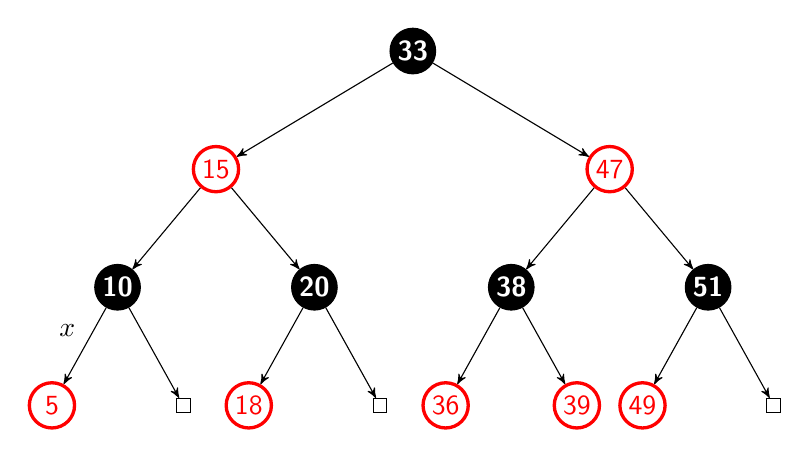
\begin{tikzpicture}[->,>=stealth',level/.style={sibling distance = 5cm/#1,
  level distance = 1.5cm}]
\node [arn_n] {33}
    child{ node [arn_r] {15}
            child{ node [arn_n] {10}
                child{ node [arn_r] {5} edge from parent node[above left]
                         {$x$}} %for a named pointer
                                                child{ node [arn_x] {}}
            }
            child{ node [arn_n] {20}
                                                child{ node [arn_r] {18}}
                                                child{ node [arn_x] {}}
            }
    }
    child{ node [arn_r] {47}
            child{ node [arn_n] {38}
                                                child{ node [arn_r] {36}}
                                                child{ node [arn_r] {39}}
            }
            child{ node [arn_n] {51}
                                                child{ node [arn_r] {49}}
                                                child{ node [arn_x] {}}
            }
                };
\end{tikzpicture}
\end{document}
